\documentclass[aspectratio=169]{beamer}

\usetheme{metropolis}
\usepackage[T1]{fontenc}
\usepackage{booktabs}
\usepackage{graphicx}
\usepackage{subcaption}
\usepackage{enumitem}
\usepackage{tikz}
\usetikzlibrary{calc}
\usepackage{multirow}

% visible bullet markers
\setbeamertemplate{itemize item}{\textbullet}
\setbeamertemplate{itemize subitem}{\textendash}
\setbeamertemplate{itemize subsubitem}{\textperiodcentered}

\setlist[itemize,1]{label=\textbullet,leftmargin=1.4em,labelsep=0.5em,itemsep=3pt,topsep=2pt,parsep=0pt}
\setlist[itemize,2]{label=\textendash,leftmargin=1.2em,labelsep=0.5em,itemsep=2pt,topsep=2pt,parsep=0pt}
\setlist[itemize,3]{label=\textperiodcentered,leftmargin=1.2em,labelsep=0.5em,itemsep=1pt,topsep=1pt,parsep=0pt}

\graphicspath{{./plots/}{../article/plots/}}

\newcommand{\code}[1]{%
  \begingroup
  \renewcommand{\_}{\textunderscore\allowbreak}%
  \texttt{#1}%
  \endgroup
}

\setbeamerfont{title}{size=\Large}

\title{A Graph-based Framework for Coverage Analysis in Autonomous Driving}
\author{Thomas Mühlenstädt \and Marius Bause}
\date{}

\begin{document}

\maketitle

% ---------------------------------------------------------
\begin{frame}{Verification and Validation Workflow}
\centering
% vv_workflow_tikz.pdf is 650x394pt (w:h ratio 650/394); the bottom-left
% band of the image (below the contribution boxes, left of the Safety Case
% box) is intentionally left blank so bullet text can sit inside it.
\newlength{\vvimgw}\setlength{\vvimgw}{0.70\textwidth}
\newlength{\vvimgh}\setlength{\vvimgh}{0.606\vvimgw}
\begin{tikzpicture}
\node[anchor=north west,inner sep=0] (vvimg) at (0,0)
  {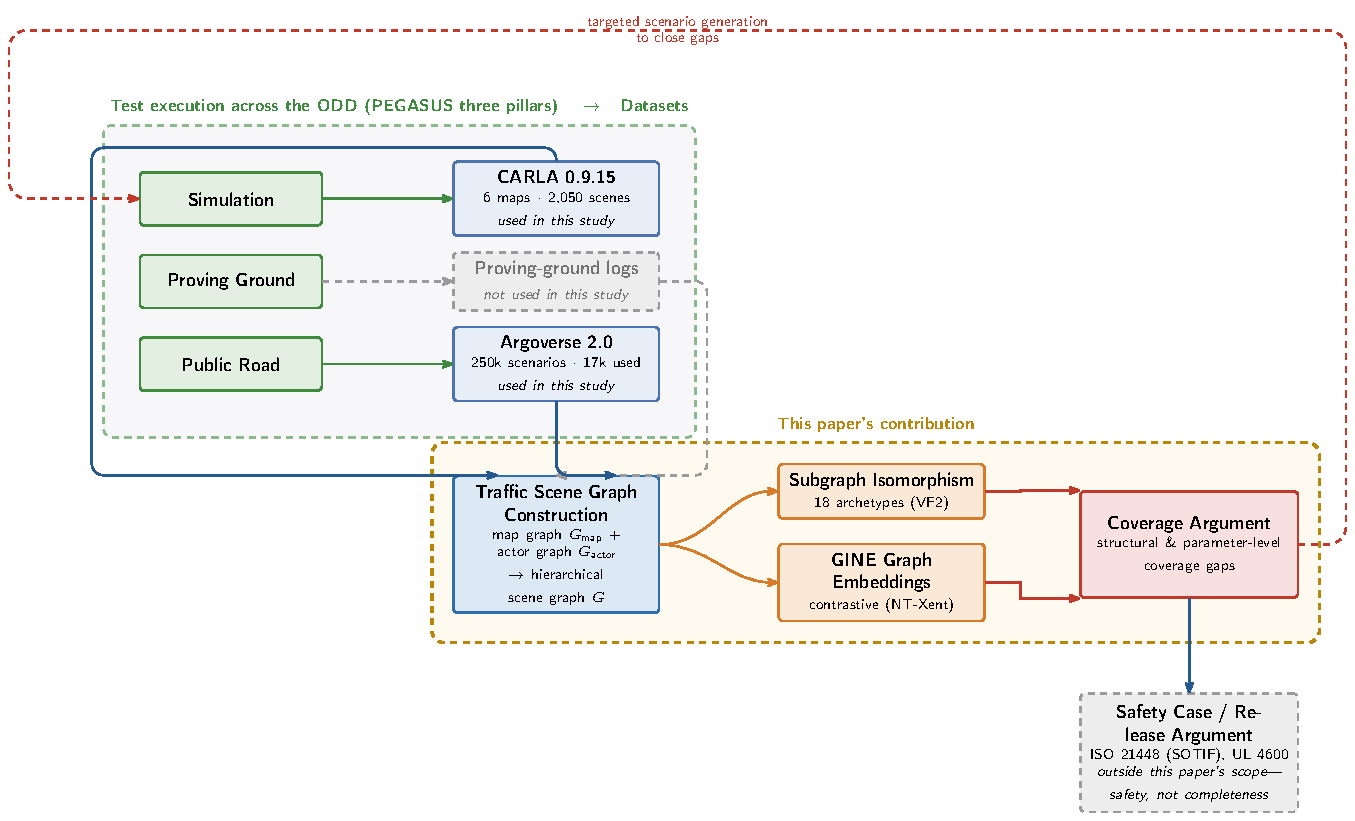
\includegraphics[width=\vvimgw]{vv_workflow_tikz.pdf}};
\node[anchor=north west,text width=0.68\vvimgw,align=left,font=\footnotesize]
  at ($(vvimg.south west)+(0.04\vvimgw,0.16\vvimgh)$)
  {\begin{itemize}
     \item CARLA (simulation), Argoverse (real-world)
     \item Ours: coverage argument via graph representation
   \end{itemize}};
\end{tikzpicture}
\end{frame}

% ---------------------------------------------------------
\begin{frame}{Hierarchical Scene Graph Construction}
\begin{columns}[t]
\begin{column}{0.48\textwidth}
    \centering
    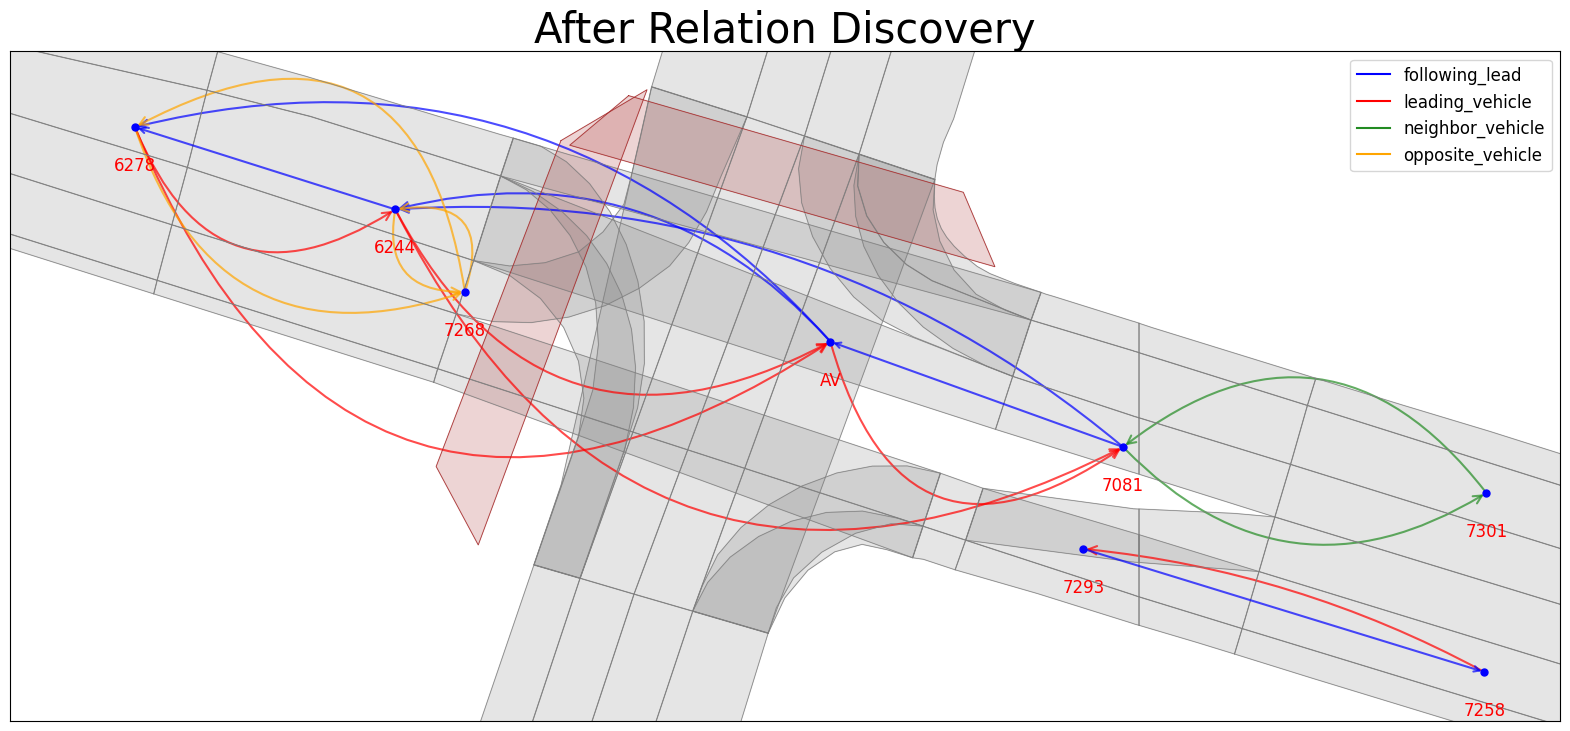
\includegraphics[width=\textwidth]{graph_construction/5758074f-be16-49da-8bb5-d43a0d8cd034_after_discovery.png}
    \\ \footnotesize After relation discovery
\end{column}
\begin{column}{0.48\textwidth}
    \centering
    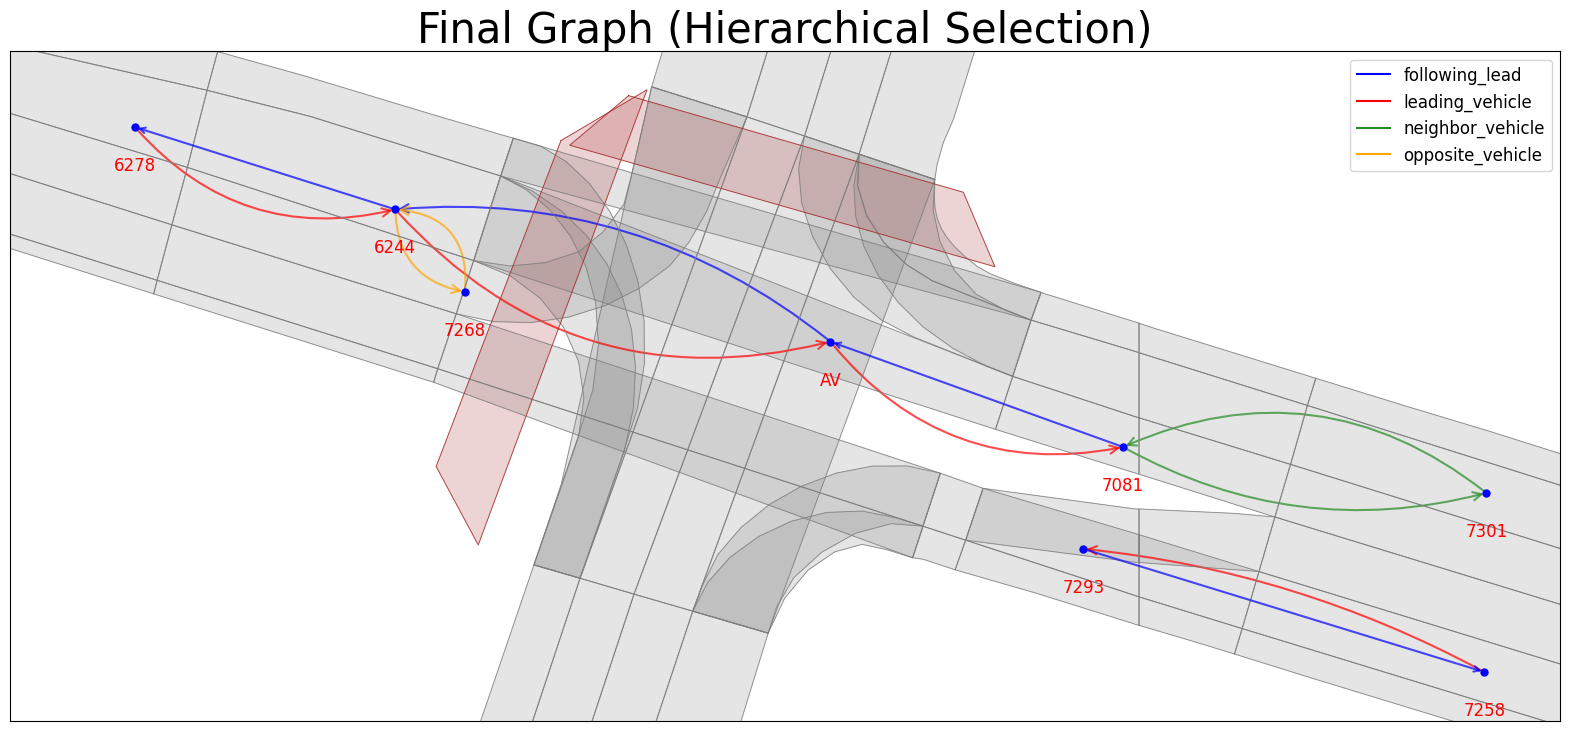
\includegraphics[width=\textwidth]{graph_construction/5758074f-be16-49da-8bb5-d43a0d8cd034_final.png}
    \\ \footnotesize After hierarchical selection
\end{column}
\end{columns}
\vspace{0.6em}
\begin{itemize}
    \footnotesize
    \item Map graph edges types included: following, neighbor, opposite
    \item Lane-change indicator: lane change within $\Delta t =1s$
    \item Phase 1 -- Relation Discovery \quad$\rightarrow$\quad Phase 2 -- Hierarchical Construction by selecting by edge type and distance
\end{itemize}
\end{frame}

% ---------------------------------------------------------
\begin{frame}{Top-Down Analysis: Scenario Archetype Coverage Gaps}
\begin{columns}[c]
\begin{column}{0.36\textwidth}
    \begin{itemize}
        \footnotesize
        \item Archetypes: 18 types user-defined (can be detected by algorithm) 
        \item Subgraph matching via the \textbf{VF2} algorithm --- near-linear in the number of nodes of the scene graph (sparse graphs)
        \item Result: missing archetypes reveal coverage gaps
    \end{itemize}
\end{column}
\begin{column}{0.62\textwidth}
    \centering
    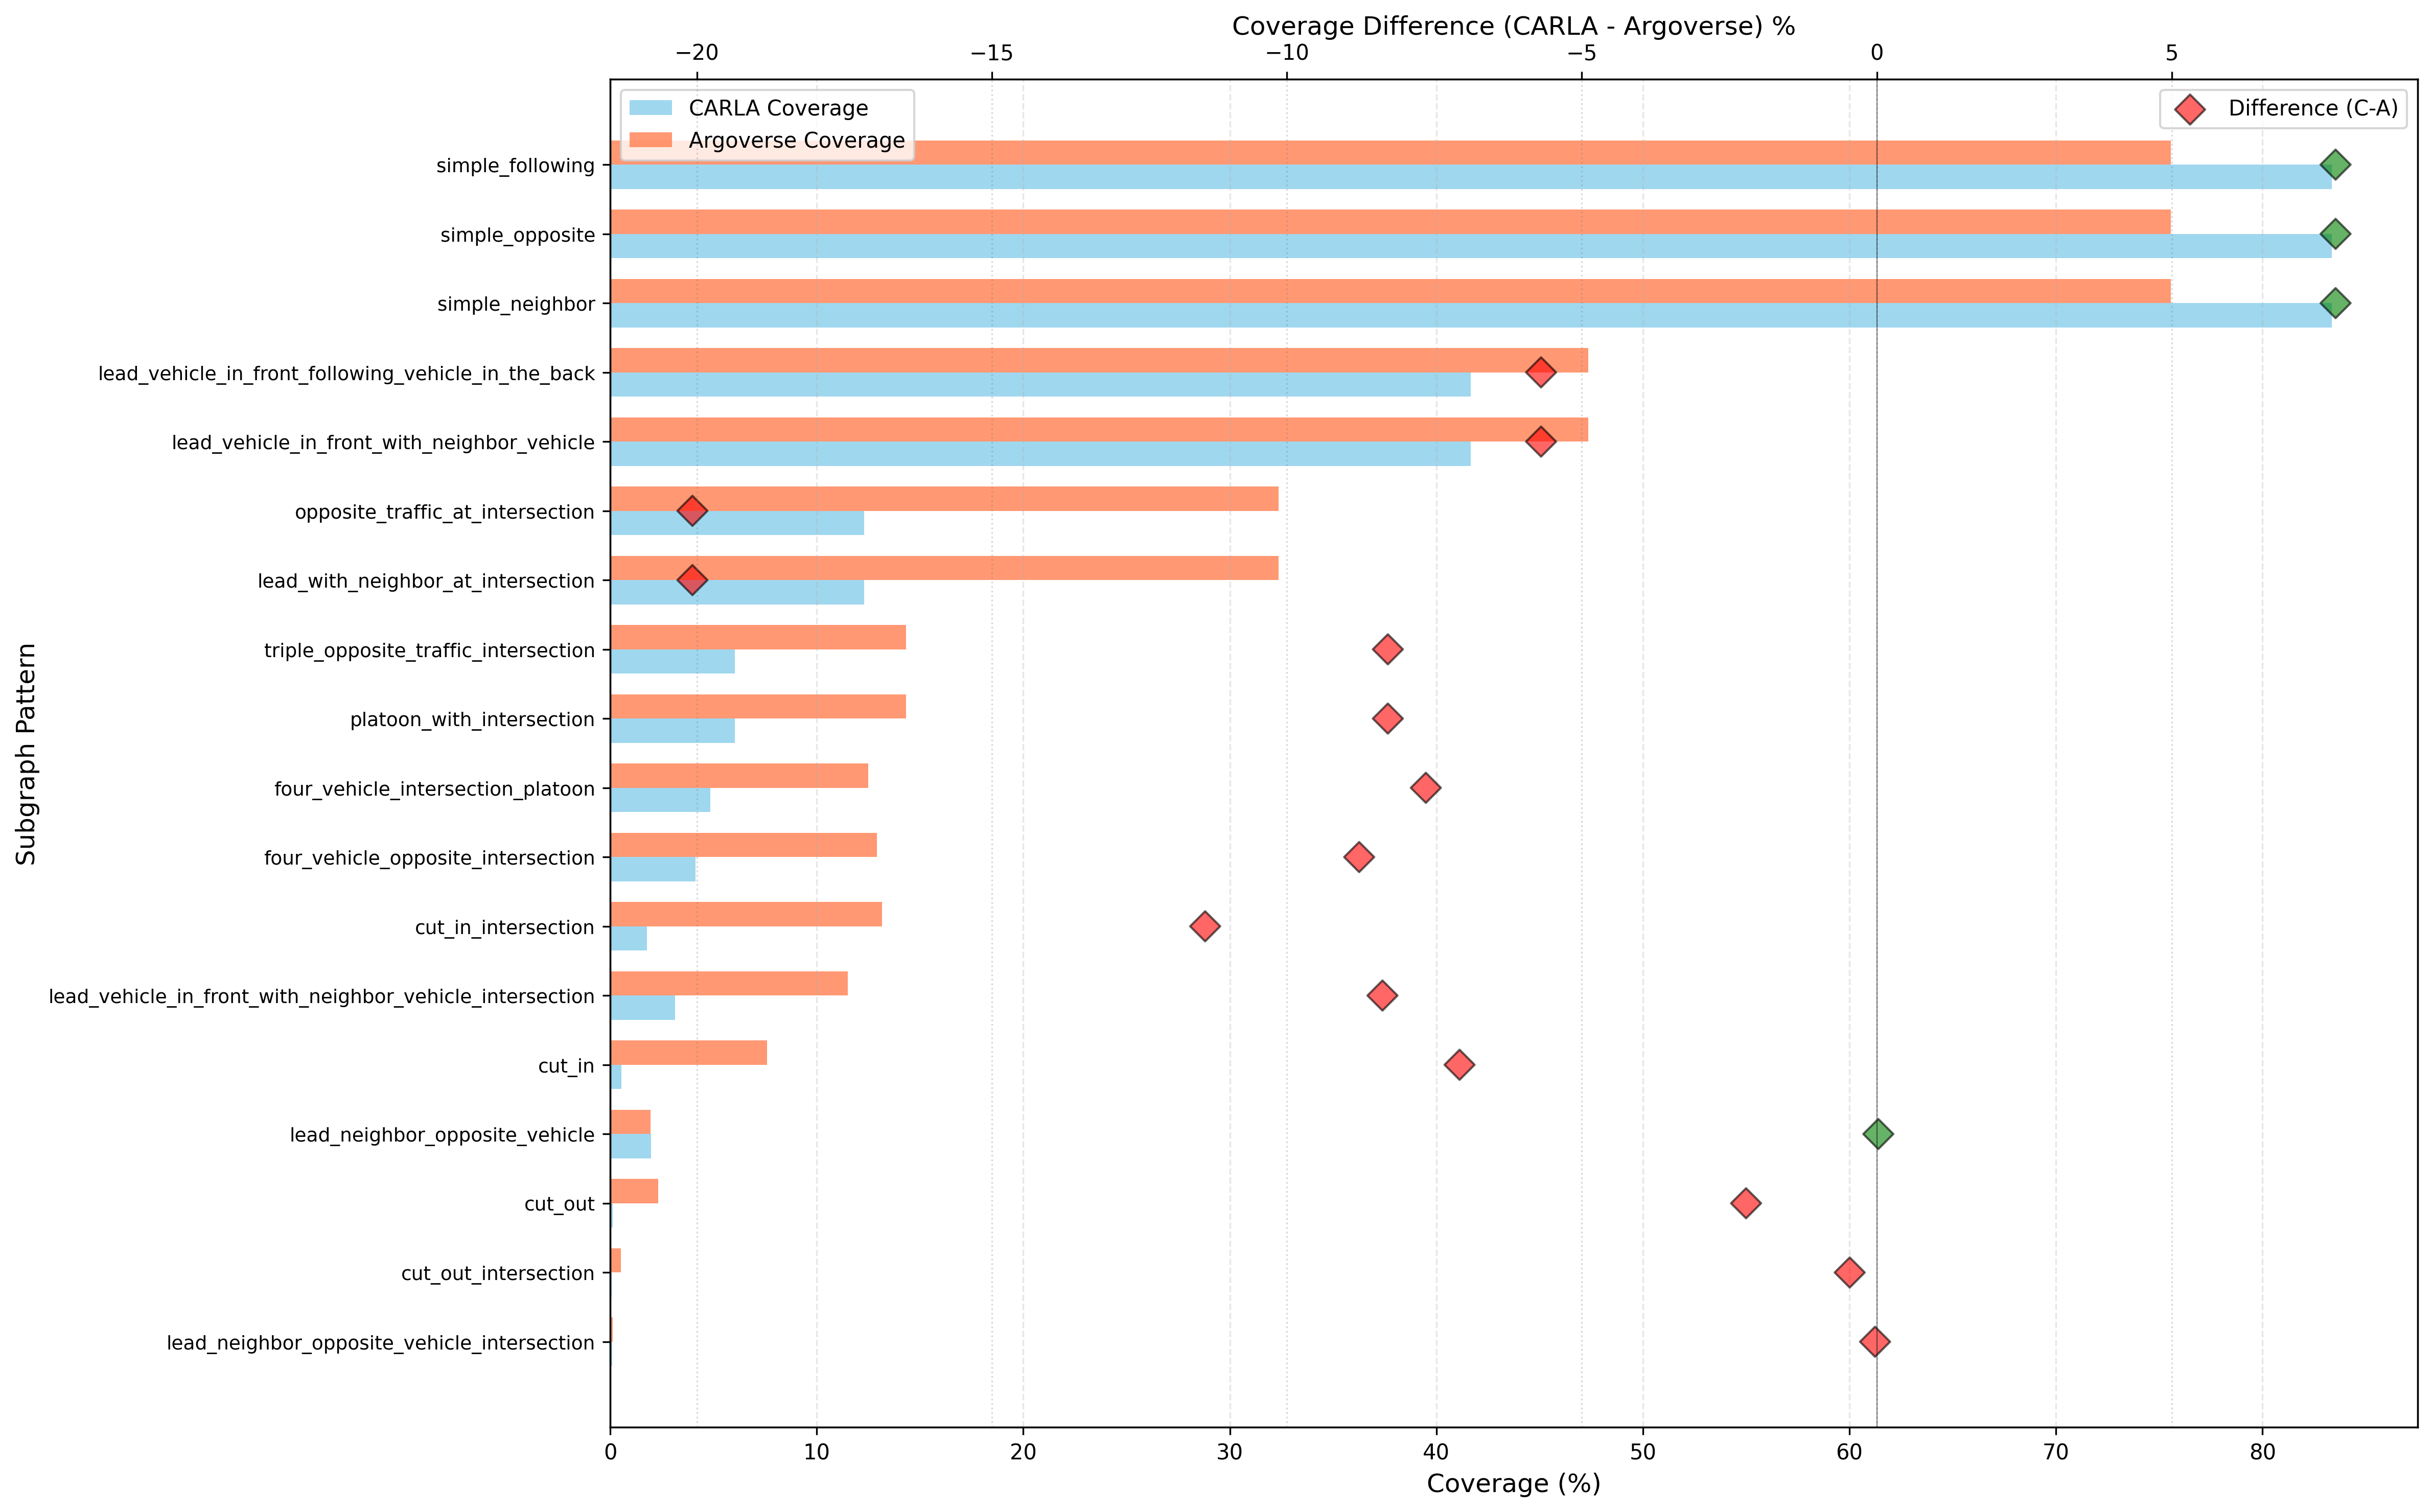
\includegraphics[height=5.8cm]{coverage_comparison_dual_axis.png}
\end{column}
\end{columns}
\end{frame}

% ---------------------------------------------------------
\begin{frame}{Bottom-Up Analysis: Embedding Space Coverage Gaps}
\begin{columns}[c]
\begin{column}{0.38\textwidth}
    \begin{itemize}
        \footnotesize
        \item \textbf{GINE}: edge-aware graph embeddings
        \item Self-supervised contrastive training (CARLA + Argoverse)
        \item Plausibility check: nearest neighbours match
        \item First 2 principal components: 40\% variance
        \item 23{,}148 Argoverse graphs flagged as gaps
    \end{itemize}
\end{column}
\begin{column}{0.60\textwidth}
    \centering
    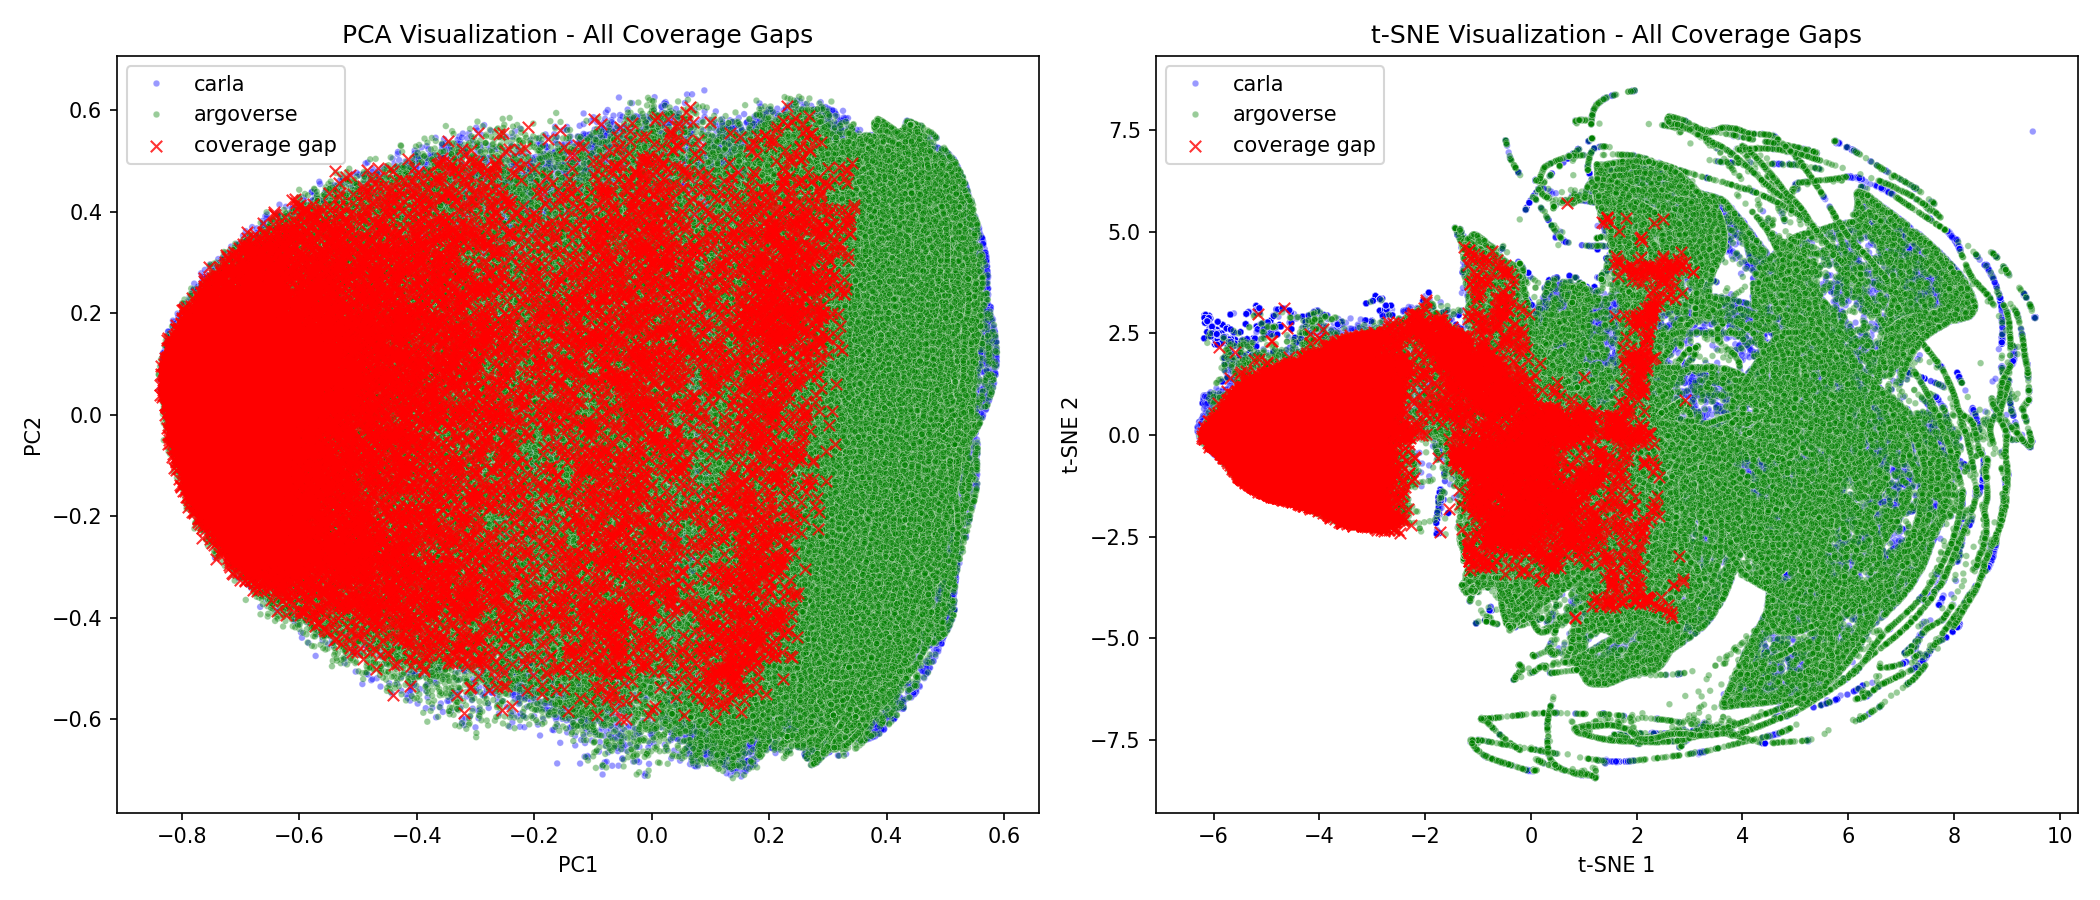
\includegraphics[width=\textwidth]{graph_embeddings_coverage_gap_visualization.png}
\end{column}
\end{columns}
\end{frame}

% ---------------------------------------------------------
\begin{frame}{Summary and Future Work}
\begin{itemize}
    \footnotesize
    \item Graph-based framework: hierarchical scene graphs combining map topology with actor relationships
    \item Two complementary coverage methods:
    \begin{itemize}
        \item subgraph isomorphism against archetypes $\rightarrow$ interpretable, pattern-based coverage
        \item GINE embeddings via contrastive learning $\rightarrow$ similarity-based coverage, clustering, anomaly detection
    \end{itemize}
    \item Validated on Argoverse 2.0 and CARLA: reveals structural, parametric, and co-occurrence coverage gaps in simulation
    \item Scales across scenarios without scenario-specific handling
    \item Naturally accommodates varying numbers of actors
    \item \textbf{Future work}:
    \begin{itemize}
        \item multi-timestep temporal graphs
        \item automatically extracting new archetype candidates from dense, unmatched embedding regions
    \end{itemize}
    \item Code: \url{https://github.com/tmuehlen80/graph_coverage}
\end{itemize}
\end{frame}

% ---------------------------------------------------------
\begin{frame}{Supplemental Material}
\centering
\vspace{2em}
{\Large Backup slides with additional graphics}
\end{frame}

% ---------------------------------------------------------
\begin{frame}{Supplement: GINE Encoder Architecture}
\centering
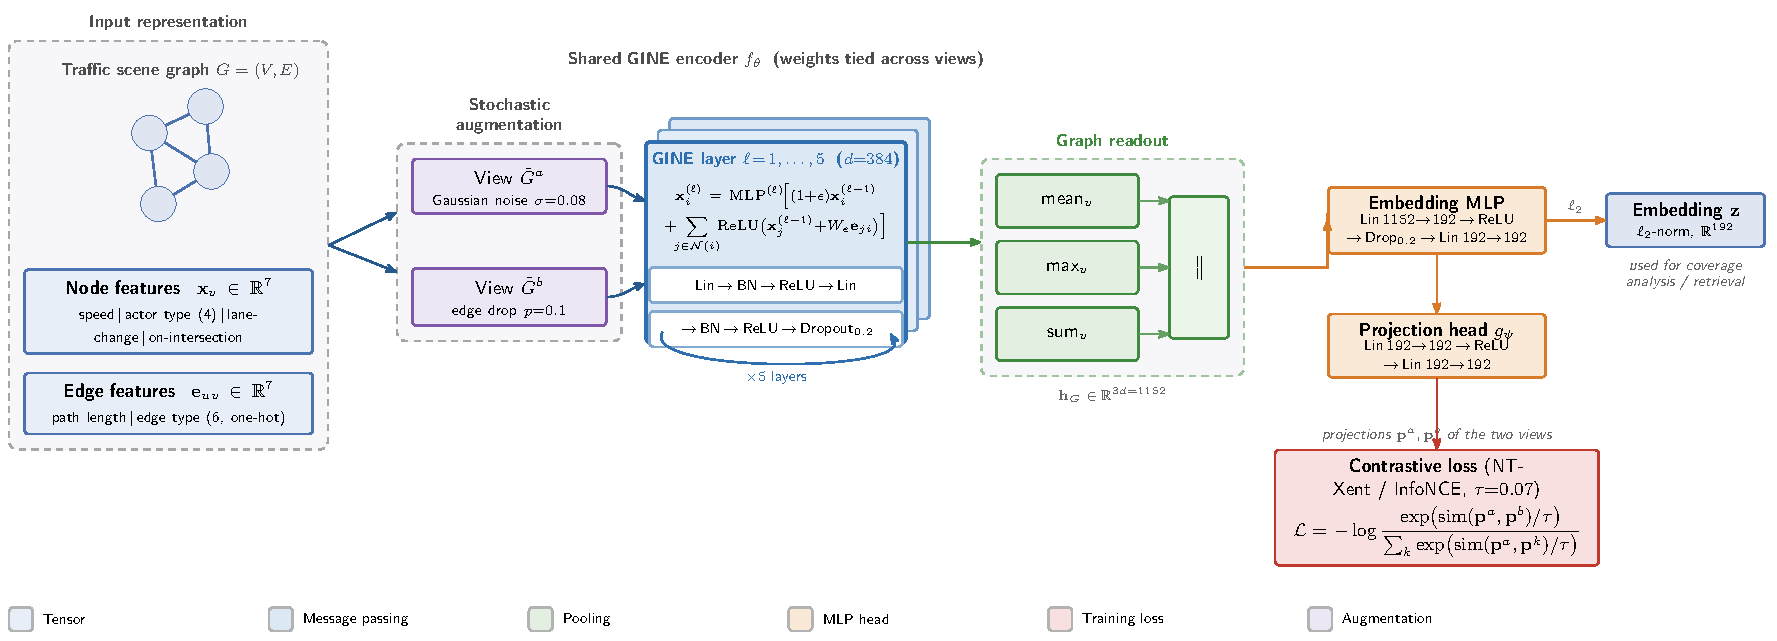
\includegraphics[width=0.85\textwidth]{graph_gine_architecture_tikz.pdf}
\end{frame}

% ---------------------------------------------------------
\begin{frame}{Supplement: Scenario Archetype Overview}
\centering
\renewcommand{\arraystretch}{0.85}
\tiny
\begin{tabular}{llccl}
\toprule
\textbf{Group} & \textbf{Archetype} & \textbf{Actors} & \textbf{Edges} & \textbf{Edge Types} \\
\midrule
\multirow{3}{*}{Simple (2-actor)}
  & Simple Following           & 2 & 2 & fl, lv \\
  & Simple Opposite            & 2 & 2 & ov \\
  & Simple Neighbor            & 2 & 2 & nv \\
\midrule
\multirow{9}{*}{Complex (3-actor)}
  & Lead + Neighbor (intersection)       & 3 & 4 & fl, lv, nv \\
  & Lead + Neighbor                      & 3 & 4 & fl, lv, nv \\
  & Cut-in                               & 3 & 4 & fl, lv \\
  & Cut-in (intersection)                & 3 & 4 & fl, lv \\
  & Platoon (intersection)               & 3 & 4 & fl, lv \\
  & Opposite Traffic (intersection)      & 3 & 4 & fl, lv, ov \\
  & Lead + Neighbor at Intersection      & 3 & 4 & fl, lv, nv \\
  & Triple Opposite (intersection)       & 3 & 4 & ov \\
  & Lead + Following in Back             & 3 & 4 & fl, lv \\
\midrule
\multirow{4}{*}{Complex (4-actor)}
  & Cut-out                              & 4 & 6 & fl, lv, nv \\
  & Cut-out (intersection)               & 4 & 6 & fl, lv, nv \\
  & 4-Vehicle Platoon (intersection)     & 4 & 6 & fl, lv \\
  & 4-Vehicle Opposite (intersection)    & 4 & 6 & fl, lv, ov \\
\midrule
\multirow{2}{*}{Complex (5-actor)}
  & Lead + Neighbor + Opposite           & 5 & 8 & fl, lv, nv, ov \\
  & Lead + Neighbor + Opposite (inters.) & 5 & 8 & fl, lv, nv, ov \\
\bottomrule
\end{tabular}
\vspace{0.5em}
\normalsize\footnotesize\\
Edge types: \textit{fl} = following\_lead, \textit{lv} = leading\_vehicle, \textit{nv} = neighbor\_vehicle, \textit{ov} = opposite\_vehicle.
\end{frame}

% ---------------------------------------------------------
\begin{frame}{Supplement: CARLA and Argoverse 2.0 Datasets}
\centering
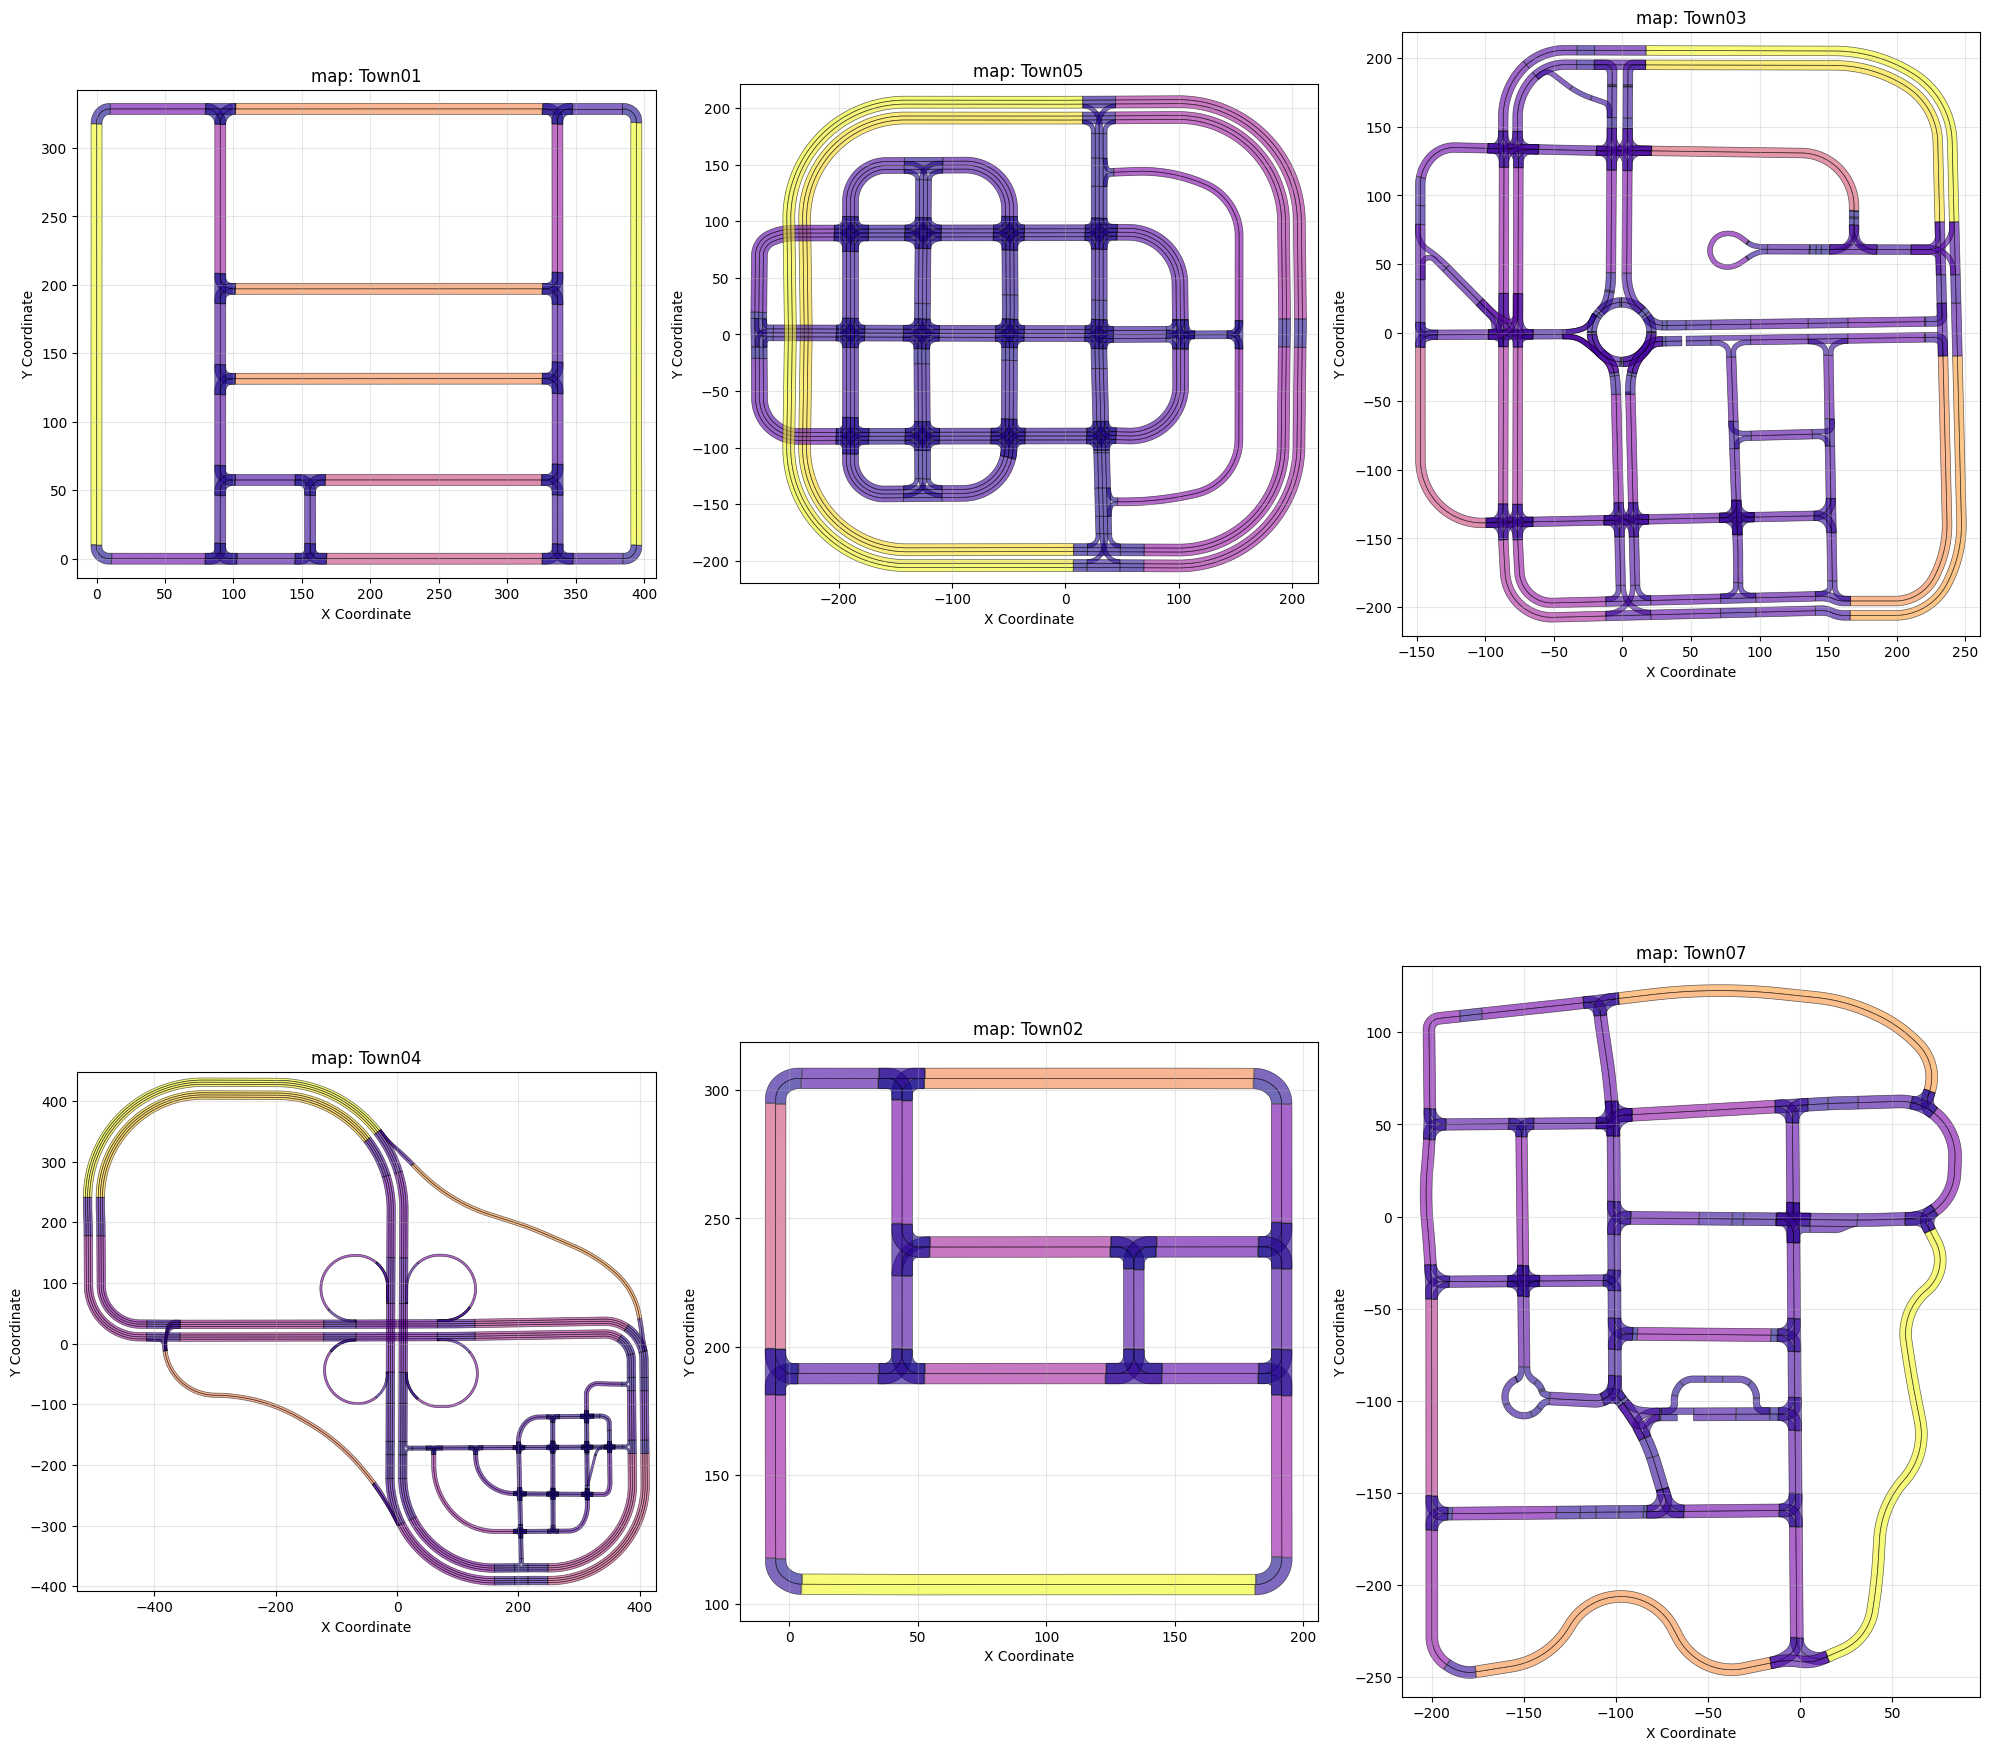
\includegraphics[width=\textwidth,height=0.48\textheight,keepaspectratio]{carla_maps_used.png}
\vspace{0.3em}
\begin{columns}[t]
\begin{column}{0.5\textwidth}
\scriptsize
\textbf{Argoverse 2.0}
\begin{itemize}[itemsep=0pt,topsep=1pt,parsep=0pt]
    \item Real-world data, 6 US cities: Austin, Detroit, Miami, Palo Alto, Pittsburgh, Washington D.C.
    \item LiDAR, ring camera imagery, HD vector maps
    \item Motion Forecasting Dataset: 250{,}000 scenarios, 11\,s each
    \item Subset used here: \textbf{17{,}000 scenes} (train partition)
\end{itemize}
\end{column}
\begin{column}{0.5\textwidth}
\scriptsize
\textbf{CARLA}
\begin{itemize}[itemsep=0pt,topsep=1pt,parsep=0pt]
    \item Version 0.9.15; maps Town01, Town02, Town03, Town04, Town05, Town07
    \item Custom generation script: trucks, motorcycles, cars with varying speed/following/lane-change behavior
    \item 20--60 vehicles per simulation run
    \item \textbf{2{,}050 scenes}, 11\,s each
\end{itemize}
\end{column}
\end{columns}
\end{frame}

% ---------------------------------------------------------
\begin{frame}{Supplement: Map and Traffic Scene Graphs}
\centering
\begin{columns}[t]
\begin{column}{0.5\textwidth}
    \centering
    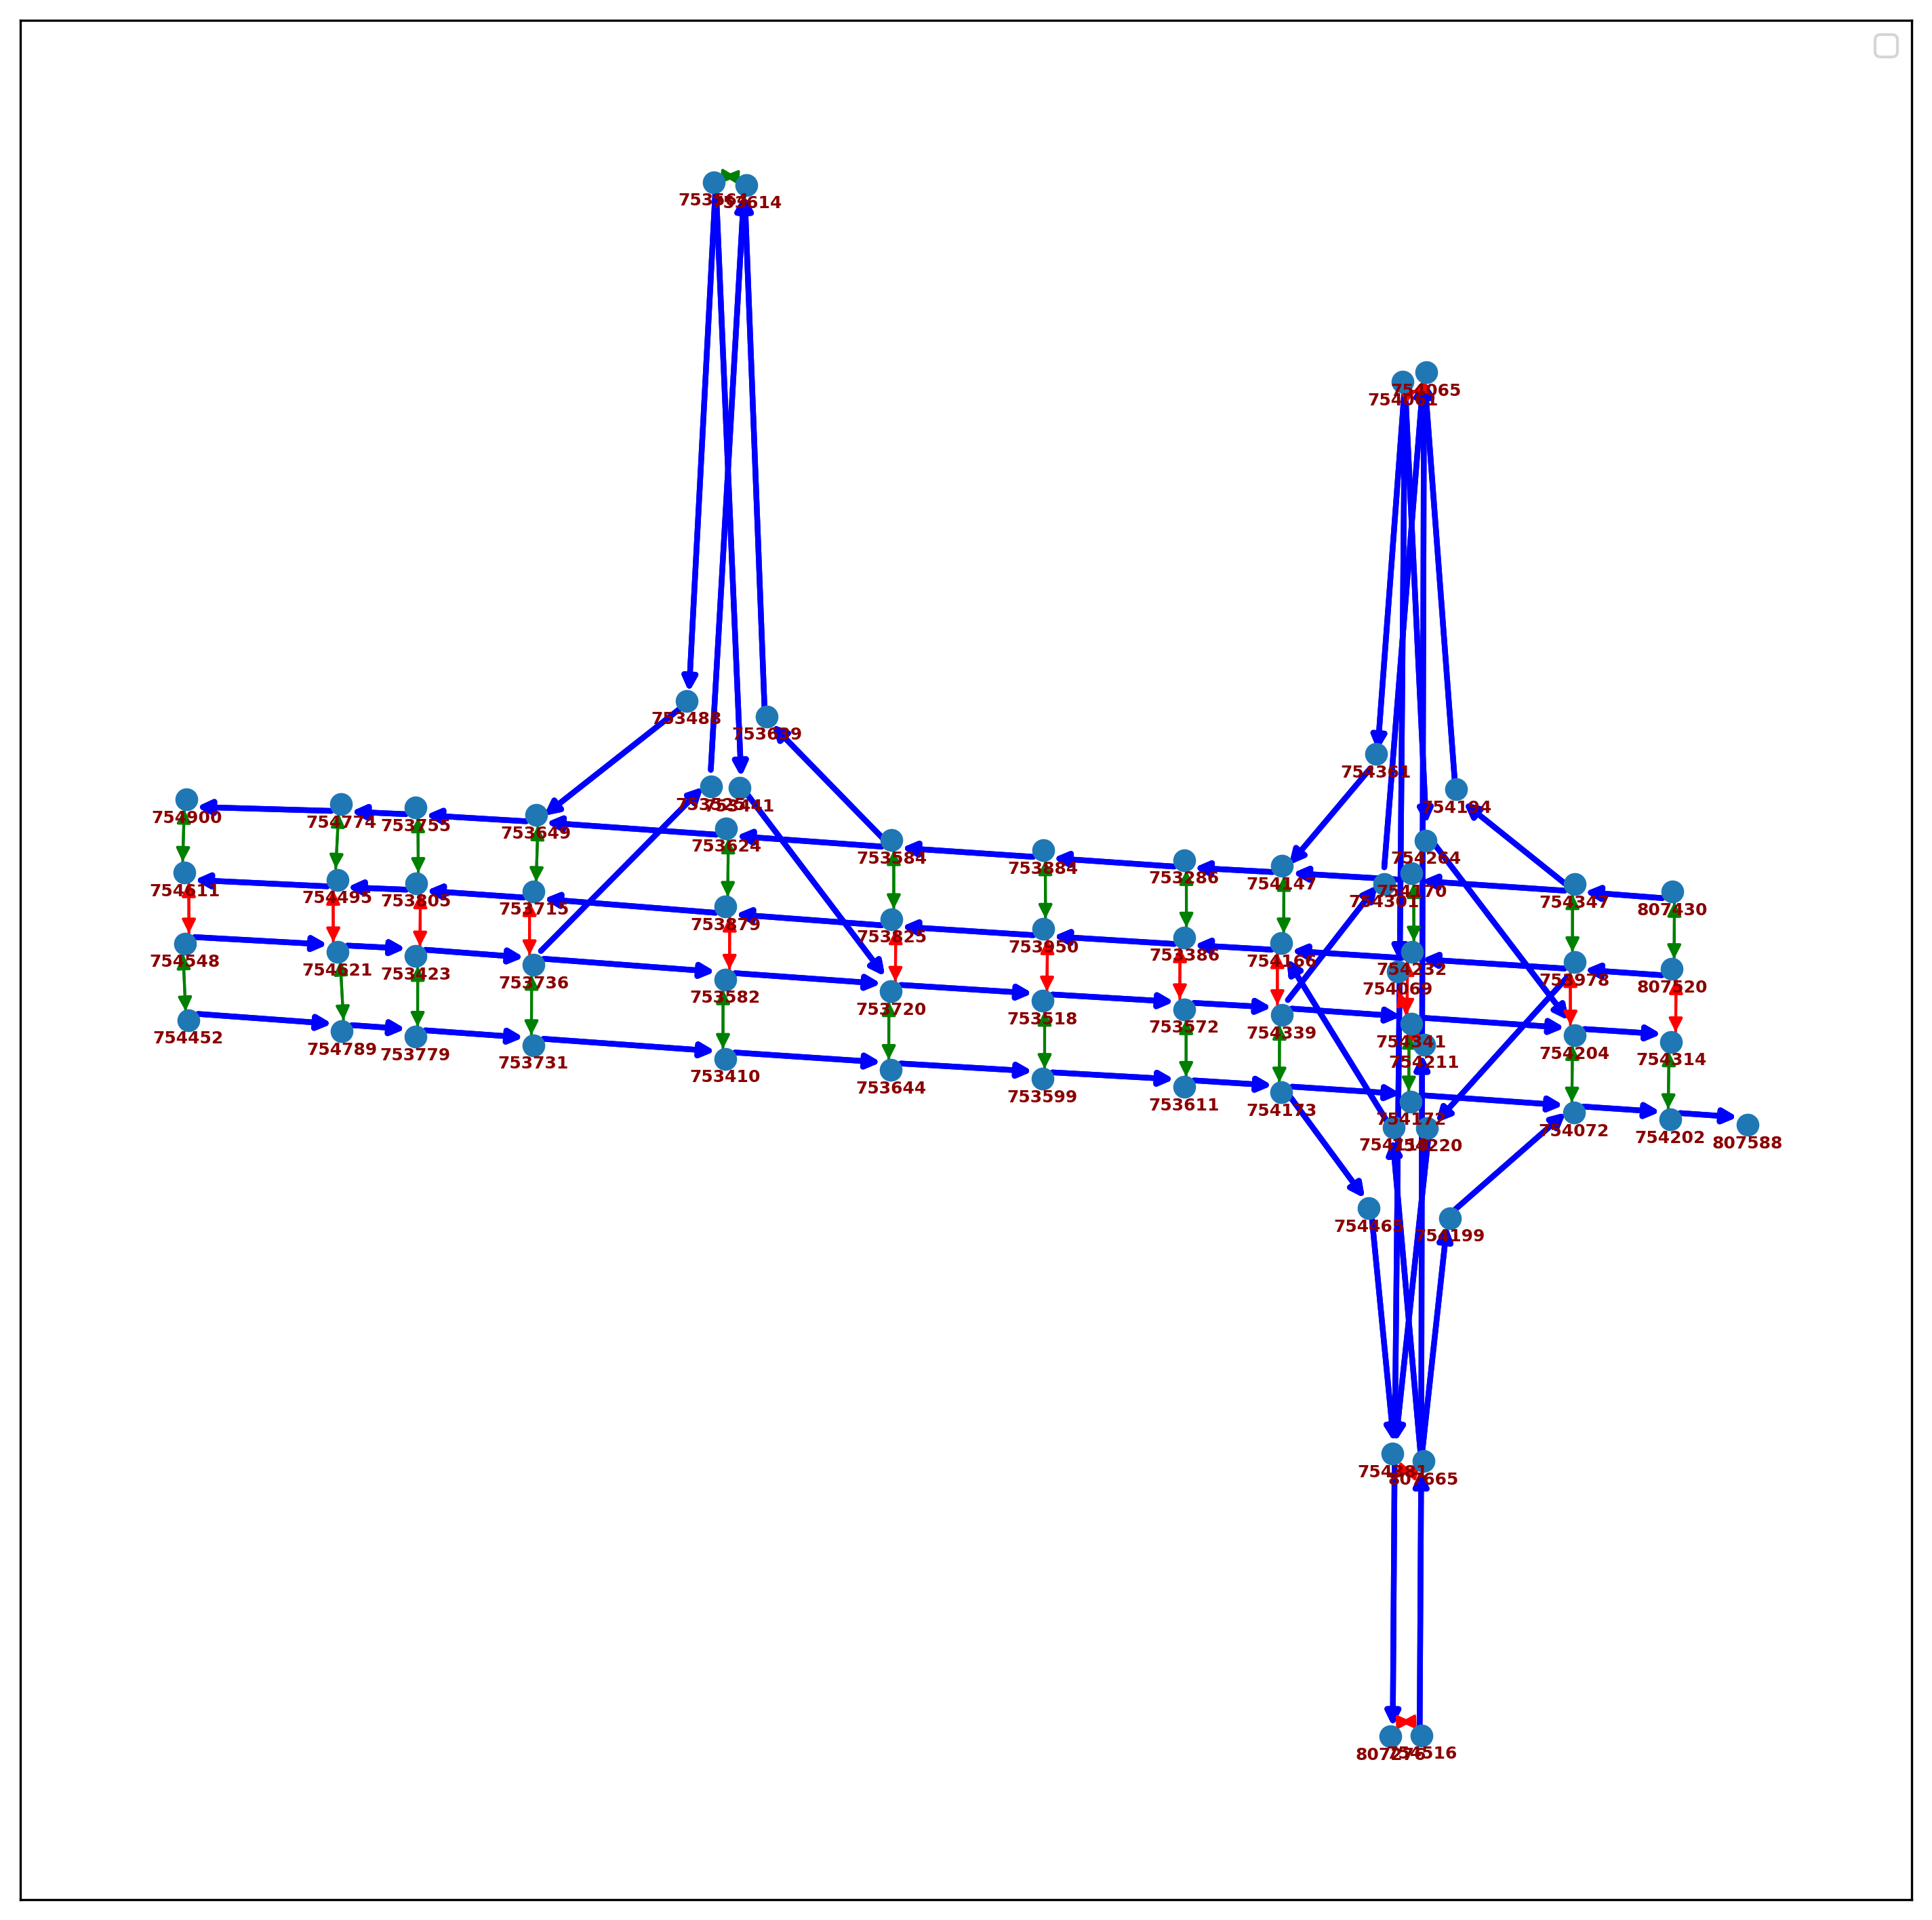
\includegraphics[width=\textwidth,height=0.62\textheight,keepaspectratio]{actor_map_graph/0922f82c-0640-43a6-b5ce-c42bc729418e_map_graph.png}\\
    \footnotesize Map graph
\end{column}
\begin{column}{0.5\textwidth}
    \centering
    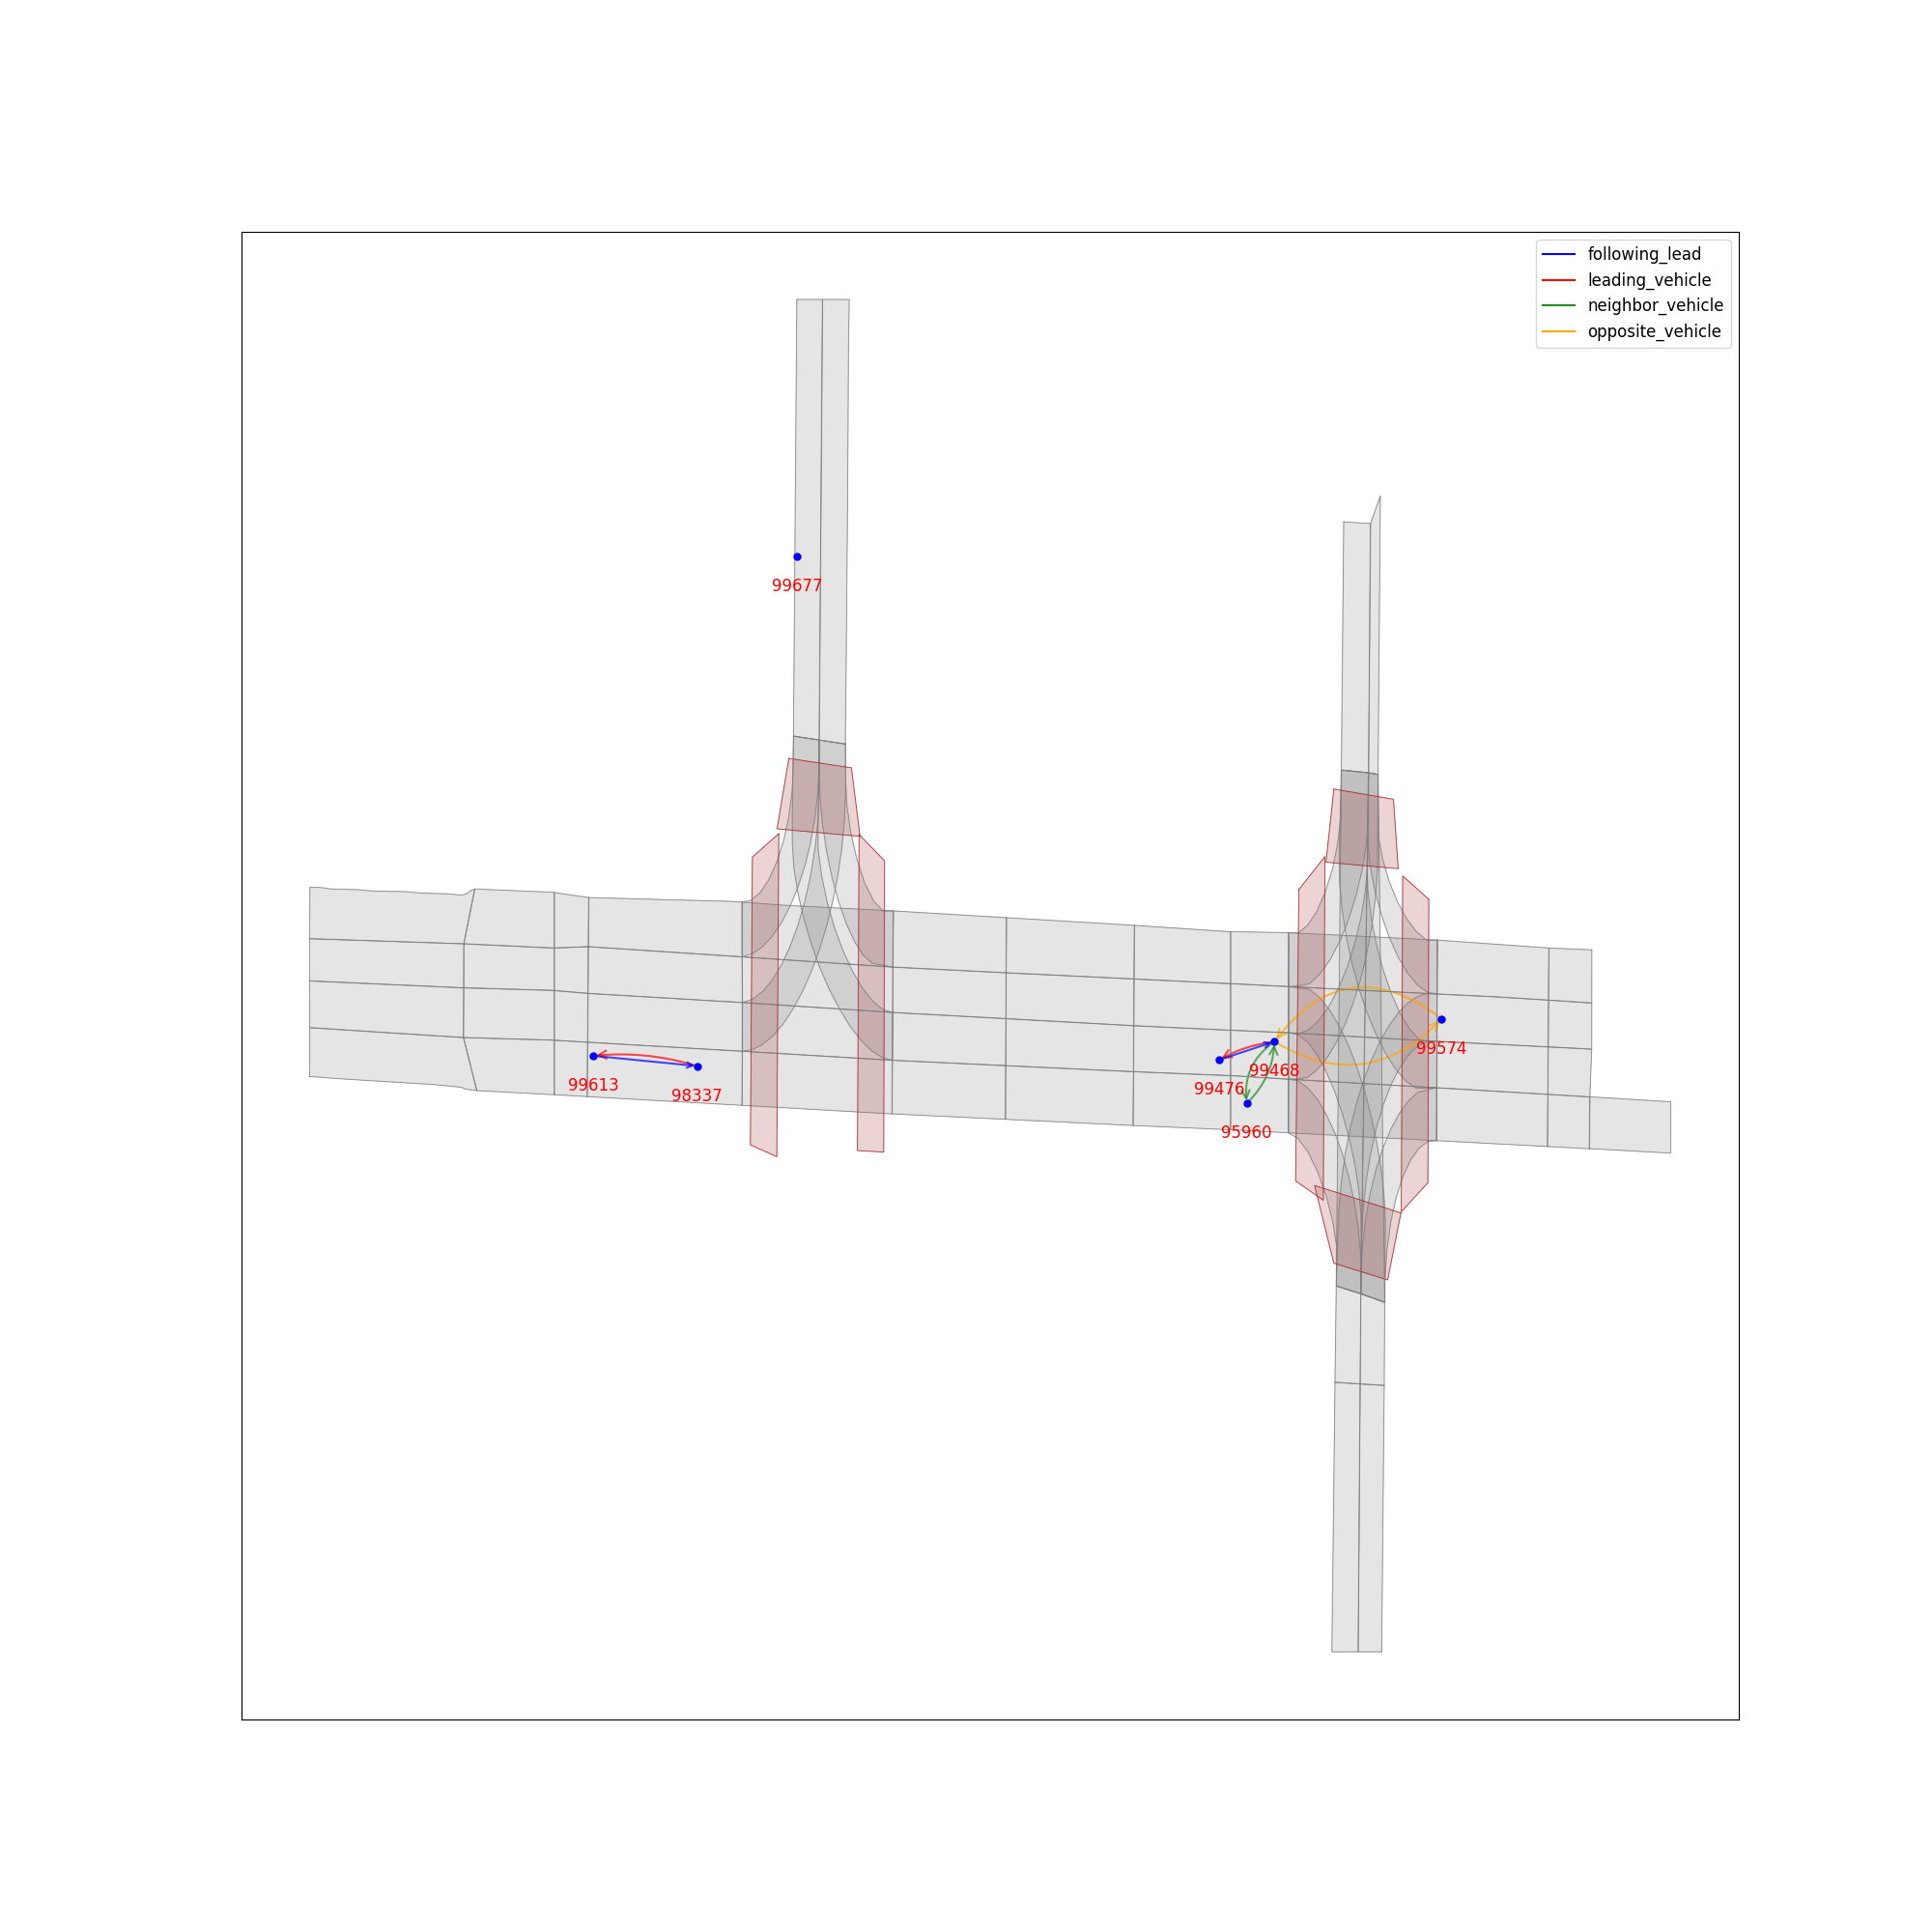
\includegraphics[width=\textwidth,height=0.62\textheight,keepaspectratio]{actor_map_graph/0922f82c-0640-43a6-b5ce-c42bc729418e_scene_at_1.0.png}\\
    \footnotesize Traffic scene graph at one timestep
\end{column}
\end{columns}
\vspace{0.3em}
\footnotesize The map graph (left) encodes spatial relationships between lanes; the traffic scene graph (right) shows actors and their relationships. Actors can be disconnected if they exceed the distance thresholds.
\end{frame}

% ---------------------------------------------------------
\begin{frame}{Supplement: Archetype Co-occurrence}
\centering
\begin{columns}[t]
\begin{column}{0.5\textwidth}
    \centering
    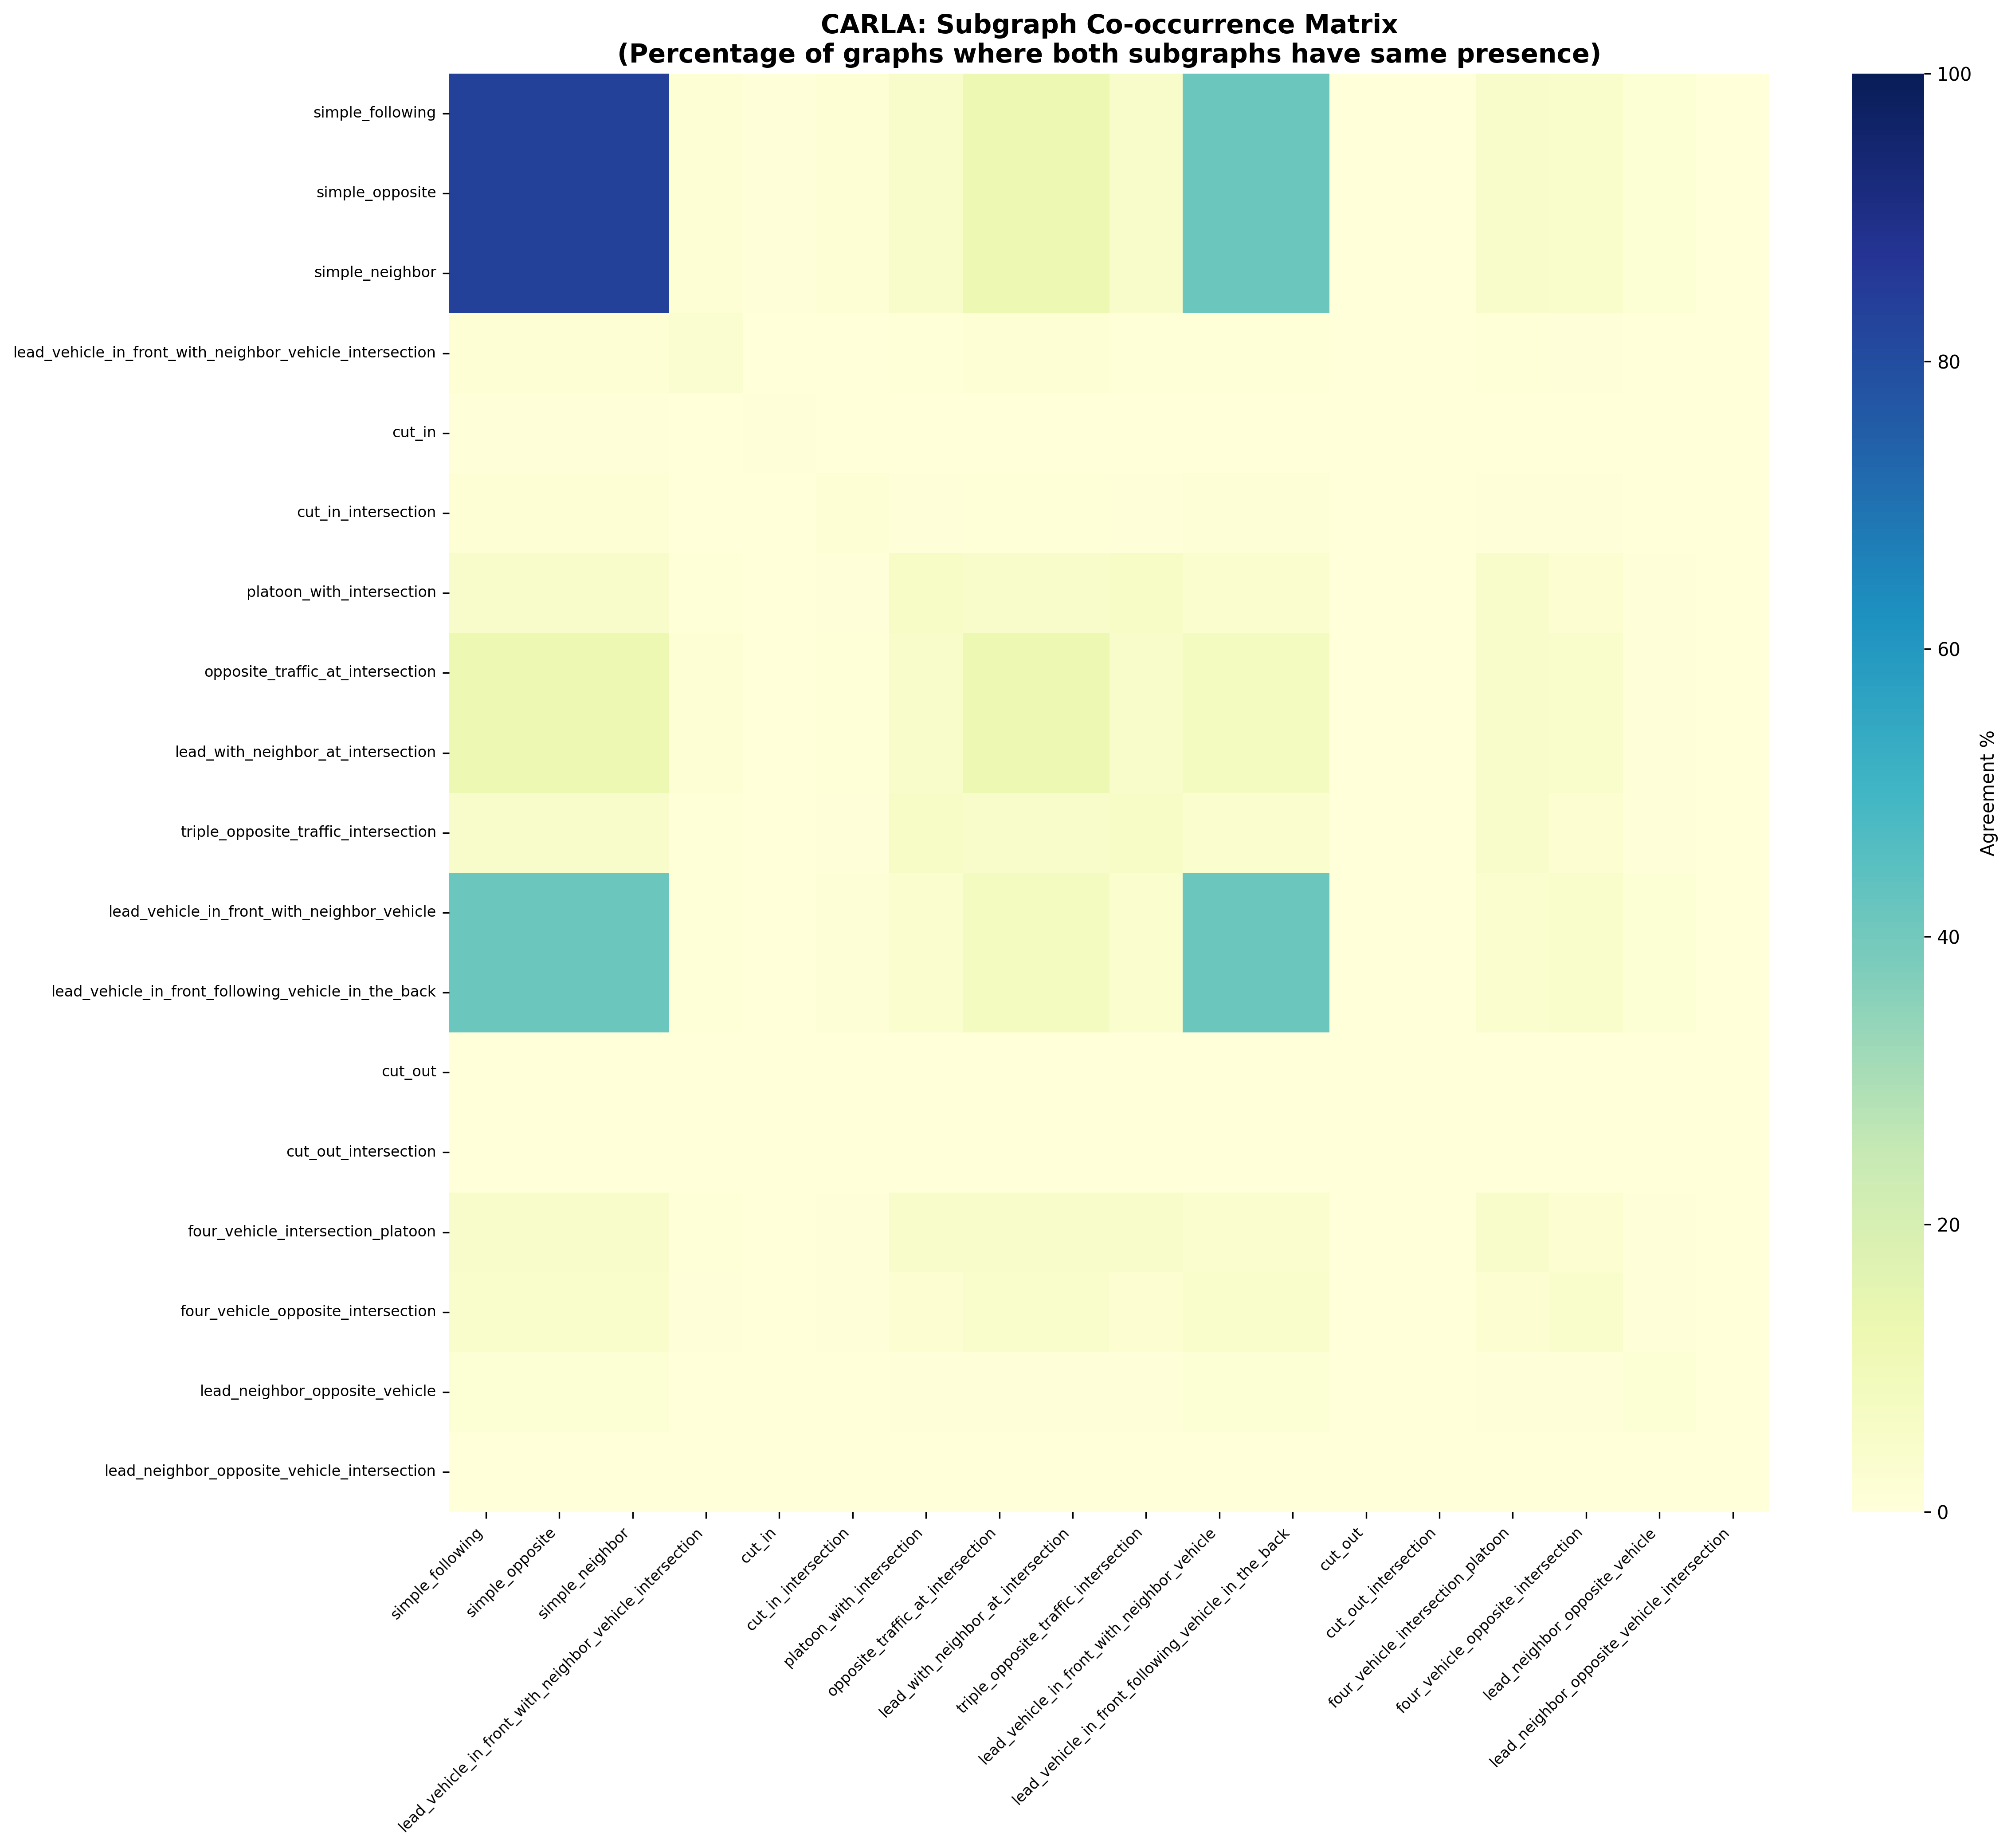
\includegraphics[width=\textwidth]{carla_agreement_matrix.png}\\
    \footnotesize CARLA
\end{column}
\begin{column}{0.5\textwidth}
    \centering
    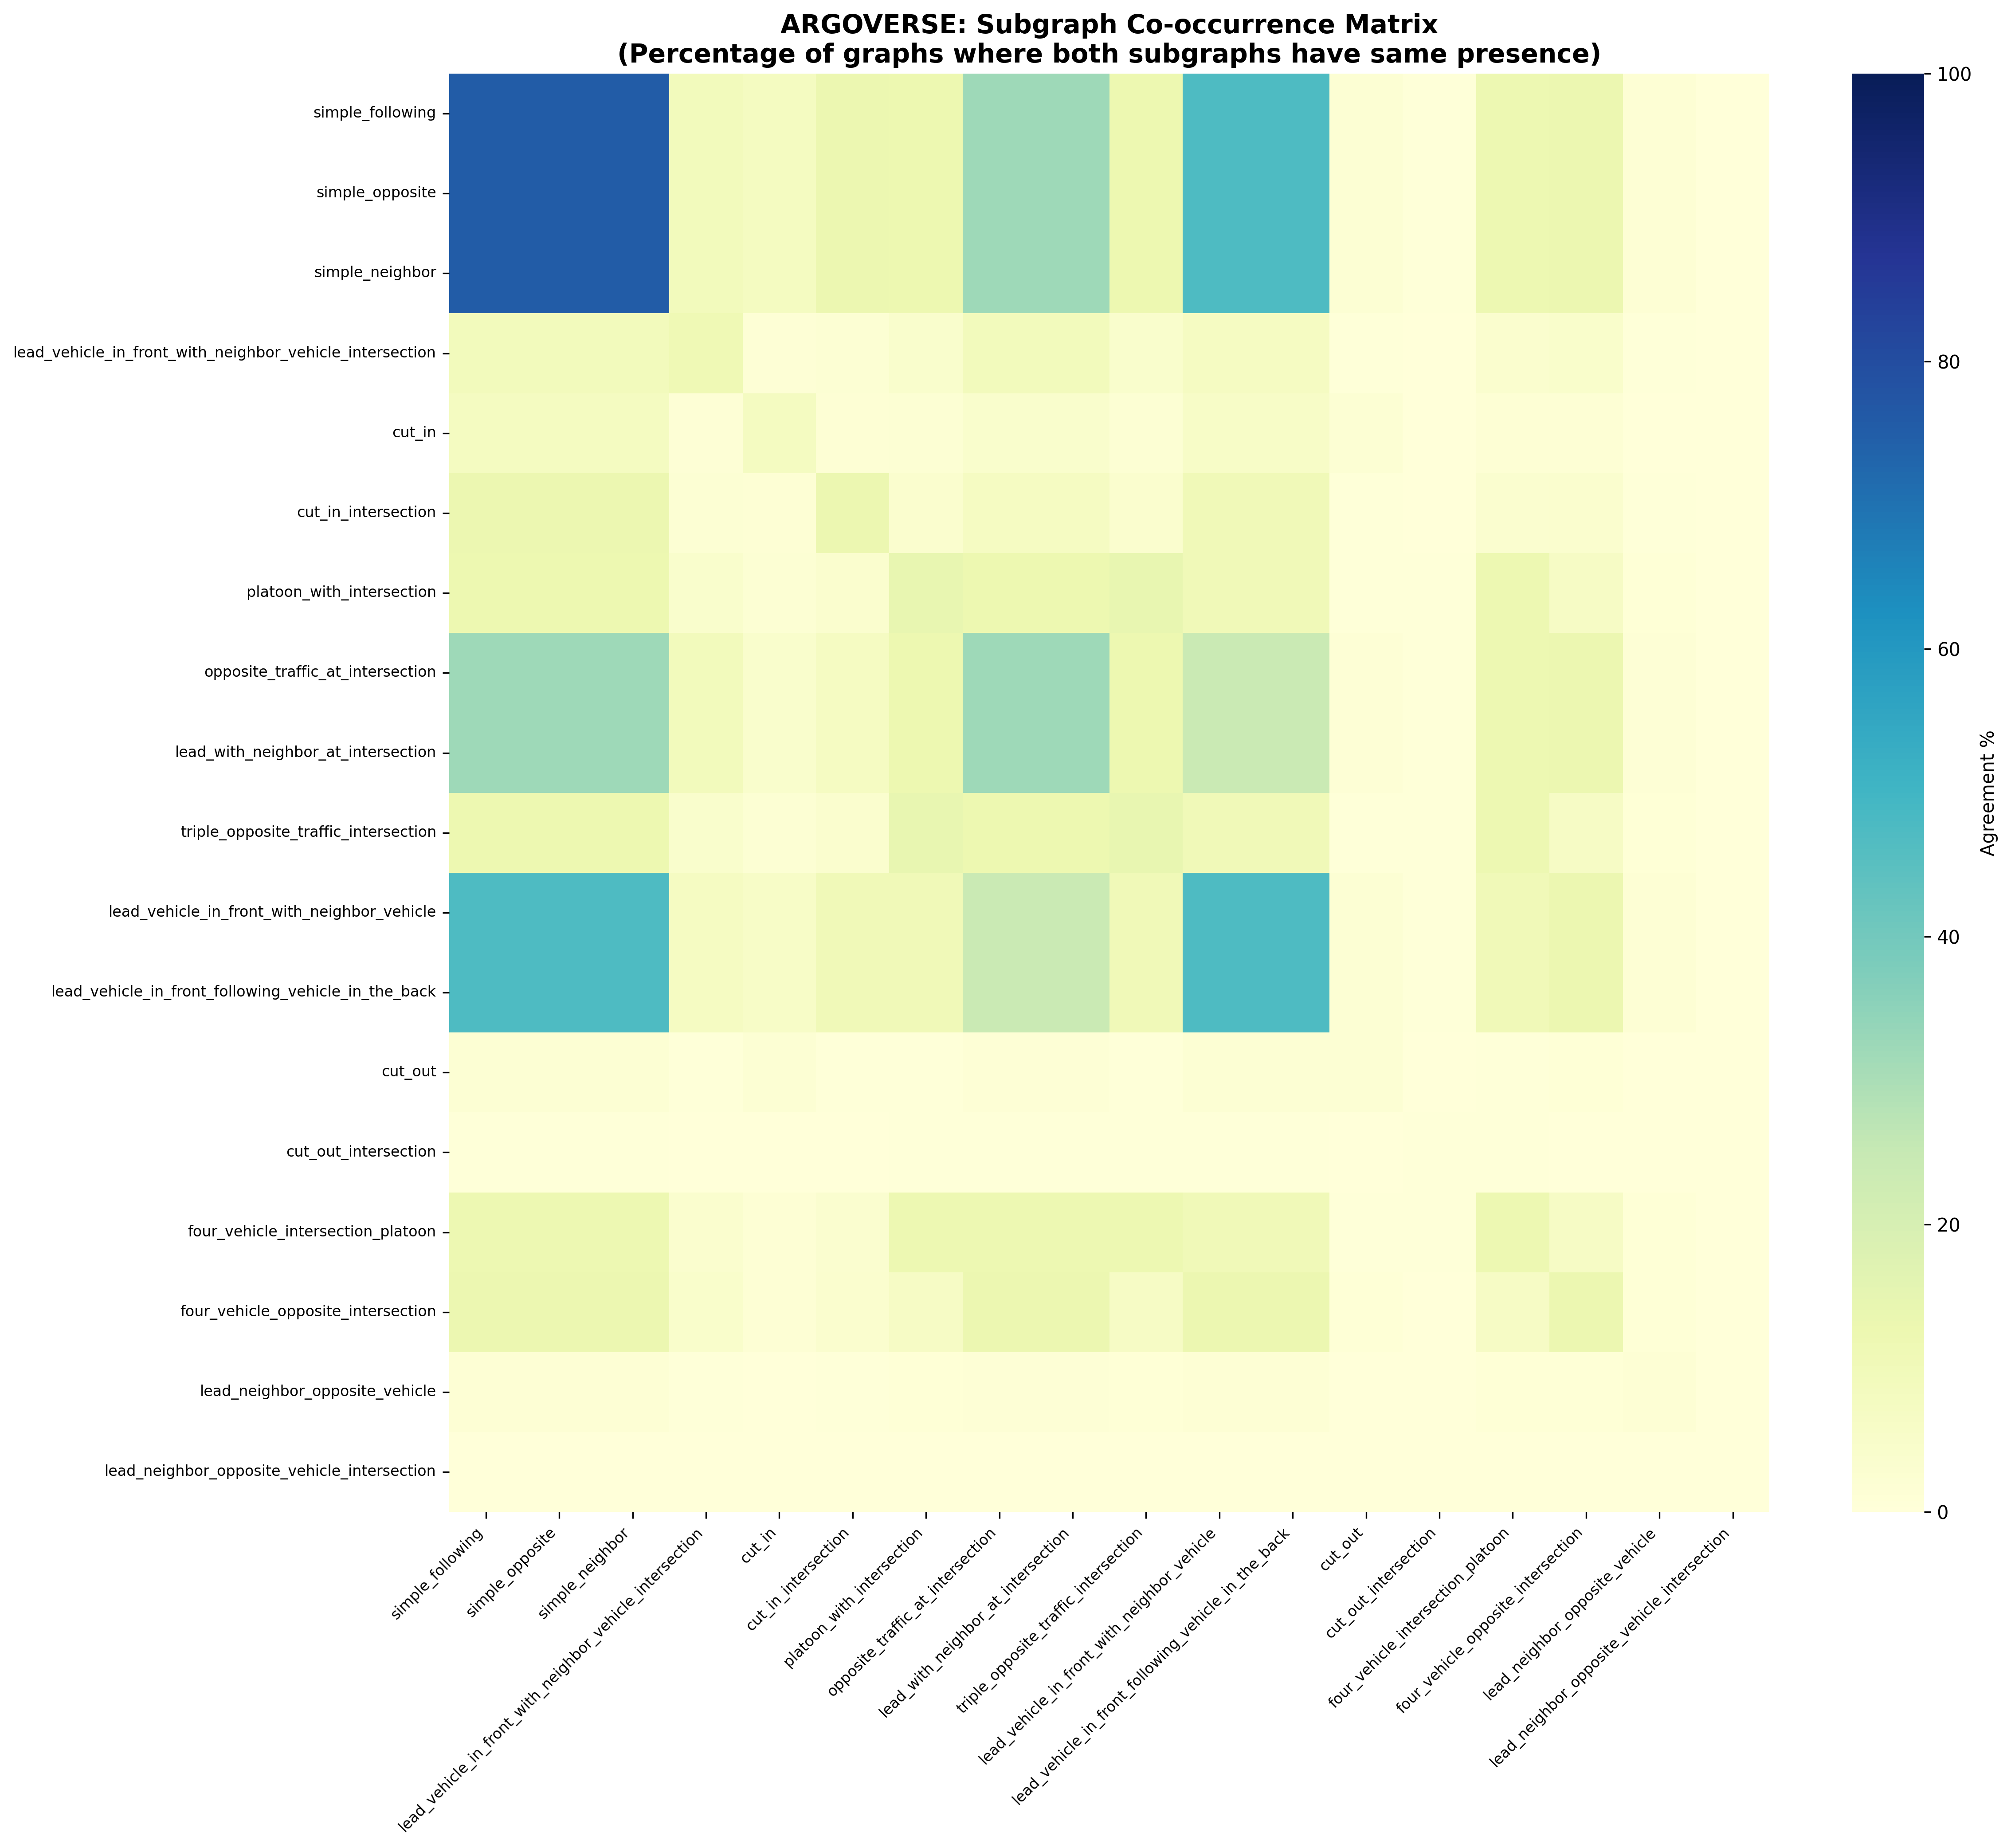
\includegraphics[width=\textwidth]{argo_agreement_matrix.png}\\
    \footnotesize Argoverse
\end{column}
\end{columns}
\vspace{0.3em}
\footnotesize Percentage of scenes in which pairs of archetypes co-occur, for CARLA and Argoverse.
\end{frame}

% ---------------------------------------------------------
\begin{frame}{Supplement: Definition Holes via Parameter Distribution}
\centering
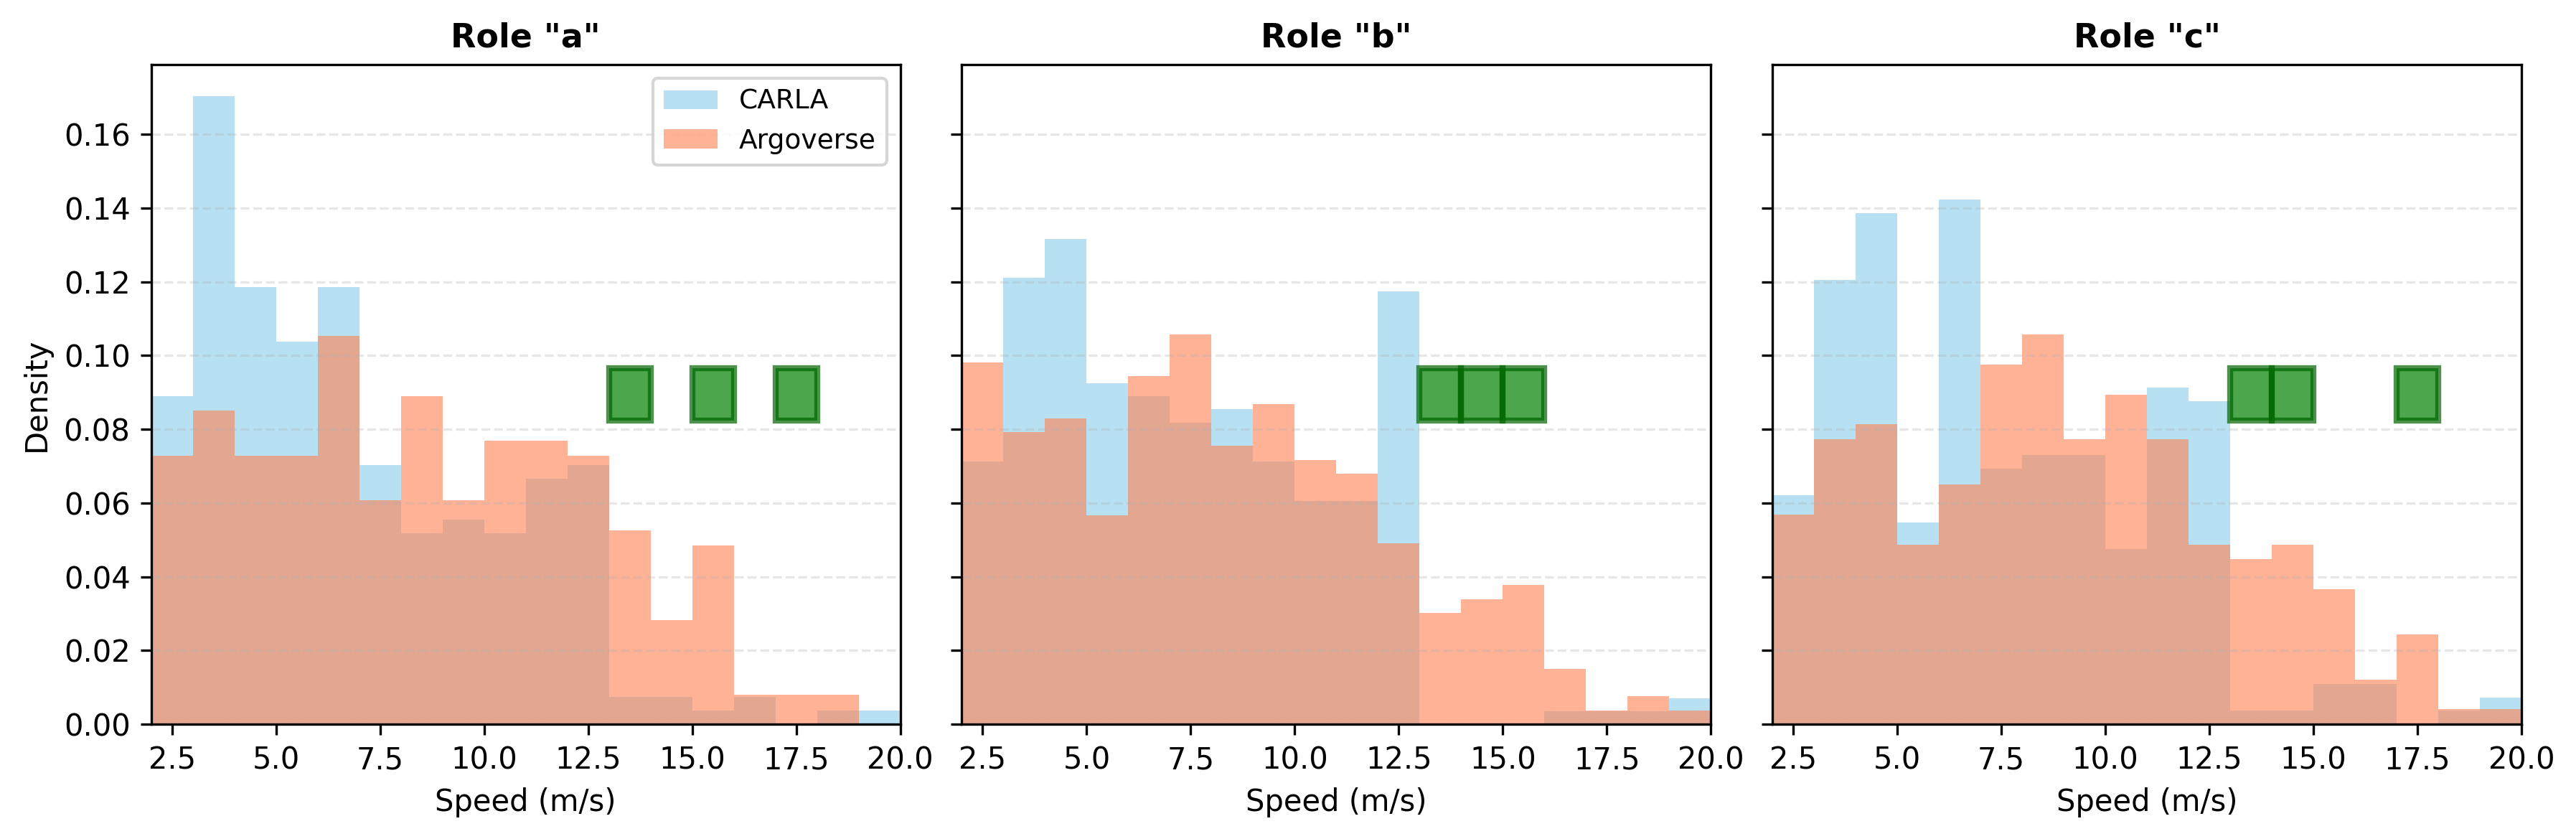
\includegraphics[width=0.85\textwidth]{role_comparison_lead_vehicle_in_front_with_neighbor_vehicle.png}
\vspace{0.3em}
\footnotesize Green rectangles mark speed ranges where Argoverse shows sufficient density but CARLA is nearly empty, for the \code{lead\_vehicle\_in\_front\_with\_neighbor\_vehicle} scenario.
\end{frame}

\end{document}
